\documentclass[14pt]{extbook}
\usepackage{multicol, enumerate, enumitem, hyperref, color, soul, setspace, parskip, fancyhdr} %General Packages
\usepackage{amssymb, amsthm, amsmath, latexsym, units, mathtools} %Math Packages
\everymath{\displaystyle} %All math in Display Style
% Packages with additional options
\usepackage[headsep=0.5cm,headheight=12pt, left=1 in,right= 1 in,top= 1 in,bottom= 1 in]{geometry}
\usepackage[usenames,dvipsnames]{xcolor}
\usepackage{dashrule}  % Package to use the command below to create lines between items
\newcommand{\litem}[1]{\item#1\hspace*{-1cm}\rule{\textwidth}{0.4pt}}
\pagestyle{fancy}
\lhead{Progress Quiz 7}
\chead{}
\rhead{Version A}
\lfoot{4173-5738}
\cfoot{}
\rfoot{Spring 2021}
\begin{document}

\begin{enumerate}
\litem{
Determine the horizontal and/or oblique asymptotes in the rational function below.\[ f(x) = \frac{6x^{2} -19 x -20}{12x^{3} +16 x^{2} -31 x -30} \]\begin{enumerate}[label=\Alph*.]
\item \( \text{Horizontal Asymptote of } y = 0.500  \)
\item \( \text{Oblique Asymptote of } y = 2x + 9. \)
\item \( \text{Horizontal Asymptote of } y = 0.500 \text{ and Oblique Asymptote of } y = 2x + 9 \)
\item \( \text{Horizontal Asymptote of } y = 0 \)
\item \( \text{Horizontal Asymptote at } y = 4.000 \)

\end{enumerate} }
\litem{
Determine the vertical asymptotes and holes in the rational function below.\[ f(x) = \frac{4x^{3} +8 x^{2} -9 x -18}{8x^{2} -22 x + 15} \]\begin{enumerate}[label=\Alph*.]
\item \( \text{Vertical Asymptote of } x = 1.25 \text{ and hole at } x = 1.5 \)
\item \( \text{Vertical Asymptotes of } x = 1.25 \text{ and } x = -1.5 \text{ with a hole at } x = 1.5 \)
\item \( \text{Holes at } x = 1.25 \text{ and } x = 1.5 \text{ with no vertical asymptotes.} \)
\item \( \text{Vertical Asymptotes of } x = 1.25 \text{ and } x = 1.5 \text{ with no holes.} \)
\item \( \text{Vertical Asymptote of } x = 0.5 \text{ and hole at } x = 1.5 \)

\end{enumerate} }
\litem{
Determine the vertical asymptotes and holes in the rational function below.\[ f(x) = \frac{9x^{3} +12 x^{2} -20 x -16}{12x^{2} -7 x -12} \]\begin{enumerate}[label=\Alph*.]
\item \( \text{Holes at } x = -0.75 \text{ and } x = 1.333 \text{ with no vertical asymptotes.} \)
\item \( \text{Vertical Asymptote of } x = 0.75 \text{ and hole at } x = 1.333 \)
\item \( \text{Vertical Asymptotes of } x = -0.75 \text{ and } x = 1.333 \text{ with no holes.} \)
\item \( \text{Vertical Asymptote of } x = -0.75 \text{ and hole at } x = 1.333 \)
\item \( \text{Vertical Asymptotes of } x = -0.75 \text{ and } x = -0.667 \text{ with a hole at } x = 1.333 \)

\end{enumerate} }
\litem{
Determine the vertical asymptotes and holes in the rational function below.\[ f(x) = \frac{16x^{3} -16 x^{2} -81 x -45}{16x^{2} -9} \]\begin{enumerate}[label=\Alph*.]
\item \( \text{Vertical Asymptote of } x = 0.75 \text{ and hole at } x = -0.75 \)
\item \( \text{Holes at } x = 0.75 \text{ and } x = -0.75 \text{ with no vertical asymptotes.} \)
\item \( \text{Vertical Asymptotes of } x = 0.75 \text{ and } x = -0.75 \text{ with no holes.} \)
\item \( \text{Vertical Asymptotes of } x = 0.75 \text{ and } x = -1.25 \text{ with a hole at } x = -0.75 \)
\item \( \text{Vertical Asymptote of } x = 1.0 \text{ and hole at } x = -0.75 \)

\end{enumerate} }
\litem{
Determine the horizontal and/or oblique asymptotes in the rational function below.\[ f(x) = \frac{9x^{3} +18 x^{2} -4 x -8}{3x^{2} -8 x + 4} \]\begin{enumerate}[label=\Alph*.]
\item \( \text{Horizontal Asymptote of } y = 2.0 \text{ and Oblique Asymptote of } y = 3x + 14 \)
\item \( \text{Horizontal Asymptote of } y = 3.0 \text{ and Oblique Asymptote of } y = 3x + 14 \)
\item \( \text{Horizontal Asymptote of } y = 3.0  \)
\item \( \text{Horizontal Asymptote at } y = 2.0 \)
\item \( \text{Oblique Asymptote of } y = 3x + 14. \)

\end{enumerate} }
\litem{
Determine the horizontal and/or oblique asymptotes in the rational function below.\[ f(x) = \frac{3x^{2} -x -10}{15x^{3} -26 x^{2} -67 x + 30} \]\begin{enumerate}[label=\Alph*.]
\item \( \text{Horizontal Asymptote of } y = 0.200 \text{ and Oblique Asymptote of } y = 5x -7 \)
\item \( \text{Horizontal Asymptote at } y = 2.000 \)
\item \( \text{Horizontal Asymptote of } y = 0.200  \)
\item \( \text{Horizontal Asymptote of } y = 0 \)
\item \( \text{Oblique Asymptote of } y = 5x -7. \)

\end{enumerate} }
\litem{
Which of the following functions \textit{could} be the graph below?
\begin{center}
    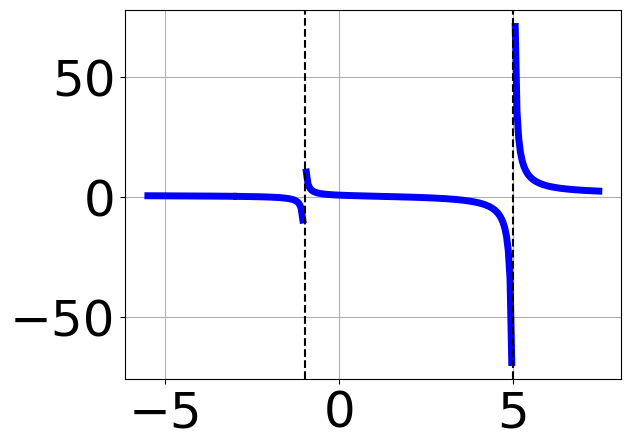
\includegraphics[width=0.5\textwidth]{../Figures/identifyGraphOfRationalFunctionA.png}
\end{center}
\begin{enumerate}[label=\Alph*.]
\item \( f(x)=\frac{x^{3} +5 x^{2} -4 x -20}{x^{3} -1 x^{2} -17 x -15} \)
\item \( f(x)=\frac{x^{3} -3 x^{2} -4 x + 12}{x^{3} + x^{2} -17 x + 15} \)
\item \( f(x)=\frac{x^{3} +3 x^{2} -4 x -12}{x^{3} -1 x^{2} -17 x -15} \)
\item \( f(x)=\frac{x^{3} -3 x^{2} -4 x + 12}{x^{3} + x^{2} -17 x + 15} \)
\item \( \text{None of the above are possible equations for the graph.} \)

\end{enumerate} }
\litem{
Determine the horizontal and/or oblique asymptotes in the rational function below.\[ f(x) = \frac{12x^{3} +25 x^{2} -48 x -45}{4x^{2} +19 x + 12} \]\begin{enumerate}[label=\Alph*.]
\item \( \text{Horizontal Asymptote of } y = 3.0 \text{ and Oblique Asymptote of } y = 3x -8 \)
\item \( \text{Horizontal Asymptote of } y = 3.0  \)
\item \( \text{Horizontal Asymptote at } y = -4.0 \)
\item \( \text{Horizontal Asymptote of } y = -4.0 \text{ and Oblique Asymptote of } y = 3x -8 \)
\item \( \text{Oblique Asymptote of } y = 3x -8. \)

\end{enumerate} }
\litem{
Which of the following functions \textit{could} be the graph below?
\begin{center}
    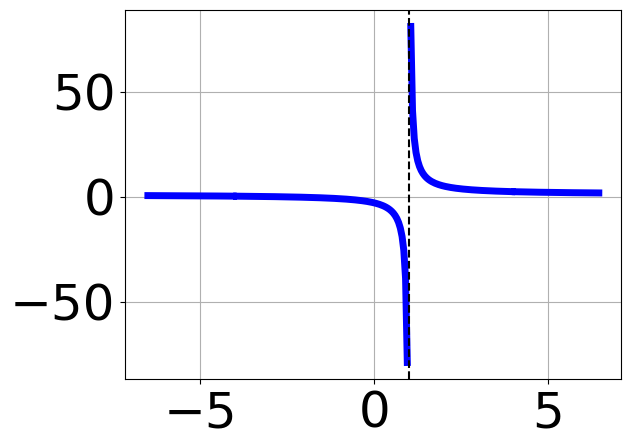
\includegraphics[width=0.5\textwidth]{../Figures/identifyGraphOfRationalFunctionCopyA.png}
\end{center}
\begin{enumerate}[label=\Alph*.]
\item \( f(x)=\frac{x^{3} +6 x^{2} +11 x + 6}{x^{3} -1 x^{2} -16 x + 16} \)
\item \( f(x)=\frac{x^{3} -3 x^{2} -16 x + 48}{x^{3} + x^{2} -16 x -16} \)
\item \( f(x)=\frac{x^{3} +3 x^{2} -16 x -48}{x^{3} -1 x^{2} -16 x + 16} \)
\item \( f(x)=\frac{x^{3} -3 x^{2} -16 x + 48}{x^{3} + x^{2} -16 x -16} \)
\item \( \text{None of the above are possible equations for the graph.} \)

\end{enumerate} }
\litem{
Determine the vertical asymptotes and holes in the rational function below.\[ f(x) = \frac{12x^{3} +53 x^{2} +57 x + 18}{16x^{2} +32 x + 15} \]\begin{enumerate}[label=\Alph*.]
\item \( \text{Vertical Asymptotes of } x = -1.25 \text{ and } x = -0.75 \text{ with no holes.} \)
\item \( \text{Vertical Asymptotes of } x = -1.25 \text{ and } x = -0.667 \text{ with a hole at } x = -0.75 \)
\item \( \text{Holes at } x = -1.25 \text{ and } x = -0.75 \text{ with no vertical asymptotes.} \)
\item \( \text{Vertical Asymptote of } x = 0.75 \text{ and hole at } x = -0.75 \)
\item \( \text{Vertical Asymptote of } x = -1.25 \text{ and hole at } x = -0.75 \)

\end{enumerate} }
\end{enumerate}

\end{document}